\documentclass[conference,a4paper]{APSIPA2018}
\usepackage{multirow}
\usepackage[dvips]{graphicx}
\usepackage{amsmath}
\usepackage[psamsfonts]{amssymb}
\usepackage{amsxtra}
\usepackage{threeparttable}

%\setlength{\voffset}{-2.0cm}
%\setlength{\hoffset}{-1cm}


\begin{document}

\title{Training Data Reduction using Support Vectors for Neural Networks}

\author{%
\authorblockN{%
Toranosuke Tanio\authorrefmark{1} and
Yanning Zhang\authorrefmark{2}
}
%
\authorblockA{%
\authorrefmark{1}
Osaka University, Osaka, Japan \\
E-mail: t-tanio@ist.osaka-u.ac.jp  Tel/Fax: +81-090-6964-9088}
%
\authorblockA{%
\authorrefmark{2}
Northwestern Polytechnical University, Xi'an, China\\
E-mail: ynzhang@nwpu.edu.cn  Tel/Fax: +86-29-XXXXXXXX}
%
}


\maketitle
\thispagestyle{empty}

\begin{abstract}
  In the field of machine learning, deep learning is widely used to 
improve versatility and accuracy by deepening the network. Deep learning 
can achieve higher expression ability compared to conventional models 
but requires large amounts of data and time for training. To tackle this 
issue, we propose a training data reduction method using support vectors 
(SVs) that are closest data to the classification boundary obtained by 
Support Vector Machine (SVM). In this research, we use the training data 
consisting of support vectors to training neural networks and evaluate 
the effect. In the evaluation experiment, we confirmed that it is 
possible to reduce the number of training data by about 12\% and reduce 
the learning time of neural network by about 9.5\% by using ResNet, a 
model of deep learning, and the CIFAR-10 data set.
\end{abstract}

\section{Introduction}
\input{intro}


\section{Related research}
This chapter describes machine learning and support vector machines as related research required to understand the proposed method. First, we will explain the components and basic principles of a neural network, which is a network model mainly used in machine learning, and then the mechanism of deep learning, which is one of machine learning methods. Next, we will describe SVM. Finally, we will talk about the existing training data reduction method.

\subsection{Machine learning}
Machine learning is a method that enables machines to learn themselves and analyze the regularity and the rule of data, instead of human beings writing all actions in the program in advance. This method makes it possible to perform specific actions by repeatedly learning and training. As an example, consider identifying images of horses and zebras. In order to identify a given image as a horse or a zebra, the machine reads a large number of images of the horse and the zebra and repeats learning. At this time, by giving instructions to pay attention to the presence or absence of the stripe pattern of the body and learning, when reading a new image of a horse or a zebra, they will be noticed and identified. As described above, it is called supervised learning that learning is performed by reading data for which answers are known in advance, which is one of the mainstream machine learning methods. Conversely, there is also unsupervised learning, but we will omit it because it is not relevant to this research.

\subsection{Neural Network}
A Neural network is a network created by mimicking the structure of the human brain. As shown in Fig. 3, it consists of nodes and synapses. Nodes are called artificial neurons, which are mathematical models created by imitating neurons in the human brain and can perform arbitrary operations. Nodes can pass computation results by connecting them, and it is the synapse used for this connection.
\begin{figure}[t]
\begin{center}
\includegraphics[width=0.6\linewidth]{fig/nn.pdf}
\end{center}
\caption{Structure of neural network.}
\vspace*{-3pt}
%{\hfill\footnotesize Note how the caption is centered in the column.\hfill}
\end{figure}


 To illustrate that neural networks can mimic the human brain's thinking circuit, as an example, we consider the question "Do you go shopping on the weekend." It is assumed that there are the following three factors as to whether to go shopping.
\begin{figure}[t]
\begin{center}
\includegraphics[width=0.8\linewidth]{fig/shopmodel.pdf}
\end{center}
\caption{Model to decide whether to go shopping.}
\vspace*{-3pt}
%{\hfill\footnotesize Note how the caption is centered in the column.\hfill}
\end{figure}
\begin{enumerate}
\item x: Closeness from home
\item y: Weather
\item z: With or without discount sale
\end{enumerate}
These outputs can be expressed as 0 or 1. For example, the output of x is one if the store is near the house, and 0 if it is far. The other two are the same. It should be noted that each factor is not an equivalent value. For example, no matter how close the store is from the house, you may never go if the weather is terrible, or even if no matter how far the store is from the house and bad the weather is, you may go if the store is making a discount sale. Such the importance of a factor is called a weight. Here, assuming that the weights of x, y and z are $w_x = 2$, $w_y = 4$ and $w_z = 8$, respectively, Fig. 4 shows a model that determines whether to go shopping. At this time, an expression indicating whether to go shopping is defined as 
\begin{equation}
xw_x+yw_y+zw_z > 5
\end{equation}
The number 5 is called the threshold, and the criterion can be changed by changing the threshold. If the threshold is 5, the shop will go shopping if it is near the house and the weather is good and if the shop is making a discount sale. In other words, if the store is near the house and the weather is good, it will go even if the store does not have a discount sale, and if it has a discount sale, other factors will be ignored. Next, assuming that the threshold is 10 and 
\begin{equation}
xw_x+yw_y+zw_z > 10
\end{equation}
if the weather is good and the store is making a discount sale, you will go shopping, and whether the store is near the house does not affect on the result. In this way, the threshold changes the criteria for deciding whether to go shopping. Although a simple network is considered in this example, if nodes are increased and more complex networks are used, more advanced judgment can be made.
 

\subsection{Deep Learning}
Deep learning is one of the machine learning methods using Deep Neural Networks (DNN). The difference between DNN and conventional neural networks is that the layers are deeply overlapped. Whereas ordinary neural networks have only one middle layer, DNN has two or more middle layers, which is a feature of DNN. Compared to ordinary neural networks, learning data, learning time, and power consumption are more massive, so that learning can be performed with higher accuracy. 
\begin{figure}[t]
\begin{center}
\includegraphics[width=0.6\linewidth]{fig/dnn.pdf}
\end{center}
\caption{Structure of Deep Neural Network.}
\vspace*{-3pt}
%{\hfill\footnotesize Note how the caption is centered in the column.\hfill}
\end{figure}
Usually, in machine learning, it is necessary to set in advance a factor called a feature that is an index of discrimination. However, in deep learning, features can be extracted automatically by updating the equation of nonlinear transformation performed in each layer. Here, as an example, Fig. 6 shows the results of identifying the spiral model. The figure represents that the orange background is positive, blue is negative, and white is 0, and the point is the data at that coordinate. From the input on the left side, it is understood that the division of the space is performed with a complicated curve each time the layer is advanced, and it is finally expressed as a spiral model.
\begin{figure}[t]
\begin{center}
\includegraphics[width=0.8\linewidth]{fig/C_SPIRAL_ReLU_L4xN8_overall.pdf}
\end{center}
\caption{General flow of feature detection.}
\vspace*{-3pt}
%{\hfill\footnotesize Note how the caption is centered in the column.\hfill}
\end{figure}
When analyzing data such as images and sounds in deep learning, the data contains many features. In order to extract this feature without loss, it is ideal for dividing it into each, but it is very defficult because the features are not always arranged at equal intervals and we do not even know what the features are at first. Therefore, it is essential to divide data without loss of features as much as possible. Here, image identification is considered as an example. If the criterion for determining whether it is kangaroo is the presence or absence of a pouch, the judgment can not be made if the portion of the pouch is on the boundary of the data division and divided into two. Thus, depending on the method of data division, features may be lost. In order to solve this, we use an overlapping method. This is a method of dividing the data by overlapping them to some extent. If it explains in the character string "abcde" for the sake of simplicity, this method is not divided into "abc" and "de" but divided into "abc", "bcd" and "cde." This can reduce the loss of features, which contributes to the increase in data analysis accuracy. 

When the data is divided and passed to each node in the first layer, the processing is performed for each node, and the data is propagated to the nodes in the next layer. At this time, each node is still in the condition that it has features required and unnecessary features(errors) to produce accurate results. If all the information is passed to the next layer, all the errors will be transmitted, and if the information passed is too small to pass the errors, the features will be lost. Here, the calculation formula applied when passing data to the next layer is called the activation function. The activation function can convey features to the next layer more clearly by slightly changing the original data, and has the effect of suppressing overfitting. There are several types of activation functions, and two primary sigmoid functions and ReLU functions are described. 

The sigmoid function is shown in Fig. 7 is a function that approaches one as the value of the input increases and approaches 0 as it decreases. The characteristic is that it is a monotonically increasing function, and it does not become one regardless of how big the original input is, and does not become -1 regardless of how small it is. The sigmoid function is shown in (3).
\begin{figure}[t]
\begin{center}
\includegraphics[width=0.8\linewidth]{fig/act.pdf}
\end{center}
\caption{Activation function.}
\vspace*{-3pt}
%{\hfill\footnotesize Note how the caption is centered in the column.\hfill}
\end{figure}
\begin{equation}
h_{sigmoid}(x)=\frac{1}{1+e^{-x}}
\end{equation}
The sigmoid function can maintain the original input characteristics to some extent but has the disadvantage that the computational complexity increases. The characteristic is that the change in value becomes gentler as it gets closer to -1 and 1, and the gradient when differentiating the sigmoid function is 
\begin{equation}
h'_{sigmoid}(x)=(1-h_{sigmoid}(x))h_{sigmoid}(x)
\end{equation}
and is almost 0 in the vicinity of those values. In other words, features tend to be flat at these values, and as the layer gets deeper, features tend to be lost, and learning may not progress. Therefore, along with the problem of computational complexity, it is often used in ordinary neural networks with few layers, but it is not often used in DNN.

In light of the shortcomings of sigmoid functions, DNN often uses the ReLU (Rectified Linear Unit) function shown in Fig. 7. The ReLU function is a function that outputs 0 when the input is 0 or less and outputs the input value as it is when 0 or more. The process is simpler than the sigmoid function, and the equation is as follows.
\begin{equation}
h_{ReLU}(x)=max(0,x)
\end{equation}
Because the ReLU function is linear, differentiation does not result in a zero gradient. As a result, there is no problem that learning will not progress due to the loss of features, which has been an issue with sigmoid functions. The calculation is also straightforward, and DNN often uses the ReLU function.

\subsection{Support Vector Machine}
Support Vector Machine (SVM) ~\cite{bib:Support-Vector-Networks} is one of pattern recognition models using supervised learning and is a method that can be used for classification and regression problems. In describing the concept of SVM, consider the problem of classifying the distribution map, as shown in Fig. 8(a). This figure is a graph representing the distribution with x as the horizontal axis and y as the vertical axis. We consider classifying orange and blue data into one hyperplane. There are many division methods, but arbitrary division methods are not possible. As an example, Fig. 8(b) shows two ways of drawing below. The two divisions are shown in Fig. 8(b) can not be regarded as incorrect because both can correctly classify orange and blue. Assuming that both lines are suitable for classification, we consider the input data shown in black. Because these input data belong to the orange side in one line and to the blue side in the other line, these lines are not suitable for classification. In this way, the data near the boundaries to be classified are vague data. SVM is a method to classify this ambiguous data as correctly as possible.
\begin{figure}[t]
  \begin{center}
    \subfigure[training data]{
      \includegraphics[width=0.48\linewidth]{fig/dist.pdf}}
      \subfigure[Classification result by difference of discrimination hyperplane.]{
      \includegraphics[width=0.48\linewidth]{fig/dist_line.pdf}}
\end{center}
\caption{Example of different classification for the same data.}
\vspace*{-3pt}
%{\hfill\footnotesize Note how the caption is centered in the column.\hfill}
\end{figure}
SVM components have support vectors and margins. The support vector is the data near the classified boundary, and the margin is the distance between the classified boundary and the data. The above vague data is data that is close to the boundary; in other words, data with a small margin. If there are many data with a small margin, the classification accuracy will be reduced, and such data can be reduced by making the margin as large as possible. This is called margin maximization. In order to prevent incorrect classification, it is only necessary to classify the data near the boundary correctly. Therefore, classification is performed by focusing on the support vectors. This concept is used in the proposed method described later. Fig. 9 shows how support vectors reduce data.
\begin{figure}[t]
  \begin{center}
    \subfigure[training data]{
      \includegraphics[width=0.35\linewidth]{data/C_XOR/inputdata2.png}}
    \subfigure[support vector]{
      \includegraphics[width=0.35\linewidth]{data/C_XOR/SVMdata2.png}}
  \end{center}
  \caption{Data reduction by support vector for XOR.}
\vspace*{-3pt}
%{\hfill\footnotesize Note how the caption is centered in the column.\hfill}
\end{figure}

\begin{figure}[t]
\begin{center}
\includegraphics[width=0.8\linewidth]{fig/dist2.pdf}
\end{center}
\caption{Example of misclassification.}
\vspace*{-3pt}
%{\hfill\footnotesize Note how the caption is centered in the column.\hfill}
\end{figure}

\begin{figure}[t]
  \begin{center}
    \subfigure[Hard margin]{
\includegraphics[width=0.45\linewidth]{fig/hardmargin.pdf}}
\subfigure[Soft margin]{
\includegraphics[width=0.45\linewidth]{fig/dist2.pdf}}
\end{center}
\caption{Hard and soft margin.}
\vspace*{-3pt}
%{\hfill\footnotesize Note how the caption is centered in the column.\hfill}
\end{figure}

Up to this point, data that can be classified finely for simplicity is taken as an example, but let us consider the case where somewhat specific data, as shown in Fig. 10, is given. If this data is classified in the same line as before, an incorrect identification will occur. Forcing correct classification of incorrectly identified data will lead to loss of these valuable data. It is called overfitting ~\cite{bib:Lessons-in-Neural-Network-Training} that it overfits the original data and the prediction accuracy for the newly given data falls. It is said that there is generalization ~\cite{bib:Generalization-in-Deep-Learning} that can be flexibly predicted for given data without causing overfitting, and tolerating an incorrect identification to some extent leads to an increase in generalization. In generalization, a technique that does not allow false identification is called a hard margin, and a technique that allows false identification to some extent is called a soft margin ~\cite{bib:An-introduction-to-kernel-based-learning-algorithms}. The soft margin allows some misidentification, but it balances the margin maximization and the allowance of the misidentification by giving a penalty. This penalty is also called cost. By adjusting the value of the cost parameter $C$, it is possible to decide how much misidentification is permitted. The following minimization problem replaces margin maximization.
\begin{equation}
\min \{\frac{1}{2}\|\beta\|^2+C\sum_{i=1}^{N}\xi_i \}
\end{equation}
$\xi$ is a slack variable, $\xi = 0$ if the data is correctly identified, $0<\xi\leq1$ if correctly identified but within the margin, and $\xi>1$ if false. That is since the second term becomes larger as there are more misidentifications, if (6) is to be minimized, an adjustment is made to reduce the value of $\xi$. It has been stated that it is possible to decide how much to allow erroneous identification by adjusting the value of the cost parameter $C$. The reason for this is the larger the value of $C$, the larger the value of the second term. Also, the case of $C \to \infty$ is called the hard margin. In the case of soft margin, adjusting the value of C can change how much incorrect identification is allowed. 

In SVM, two kernel methods, RBF (Radial Basis Function) kernel and polynomial kernel, are widely used for classification. The kernel method is a data analysis method developed from the 1990s when the proposal of SVM started, and it is a convenient method when dealing with nonlinear data. As an example, circularly distributed nonlinear data, as shown in Fig. 12(a) cannot be classified linearly.
\begin{figure}[t]
  \begin{center}
    \subfigure[Example of data that can not be classified linearly]{
      \includegraphics[width=0.48\linewidth]{fig/circle.pdf}}
    \subfigure[Convert to data that can be classified linearly]{
        \includegraphics[width=0.48\linewidth]{fig/transcircle.pdf}}
\end{center}
\caption{Transformation of nonlinear data by kernel method.}
\vspace*{-3pt}
%{\hfill\footnotesize Note how the caption is centered in the column.\hfill}
\end{figure}
\begin{equation}
(z_1,z_2,z_3) = (x^2,y^2,\sqrt{2}xy)
\end{equation}
By using the kernel method for coordinate conversion, data that cannot be classified linearly can be converted to data that can be classified linearly. The following equation represents the RBF kernel of the two kernels used in my evaluation. 
\begin{equation}
K_p(x_i,x_j) = \exp(-\gamma\|x_i-x_j\|^2)
\end{equation}
The RBF kernel is a frequently used kernel function and often uses $C$ and $\gamma$ as hyperparameters of SVM. Next, the equation for the polynomial kernel is as follows.
\begin{equation}
K_p(x_i,x_j) = {x_ix_j+r}^{d}
\end{equation}
This is a kernel represented by a polynomial of order $d$, with $r$ added as a hyperparameter. Sections 3 and 4 show how effective these two kernel functions are for reducing training data. 

\subsection{Training data reduction method}
We consider two existing studies on training data reduction. The first is a study by Nguyen et al. using support vectors to examine how training data reduction and classification accuracy change with two-dimensional data ~\cite{bib:Support-Vector-Machines-Data-Reduction-and-Approximate-Kernel-Matrices}. This study describes the trade-off between classification accuracy when data reduction is performed using support vectors, and the problem of classifying three different data distributions: Gaussian, sine, and an ellipse, which are two-dimensional data. This derives an upper limit on how much data reduction is possible by the support vector, and it has been shown that training data can be reduced by an appropriate amount within a predetermined tolerance range. It is found that the reduction of training data by support vectors is effective in classification problems of 2D data.

 Next, as the second existing study, we describe training data reduction using support vectors for neural networks conducted by Dahiya et al. ~\cite{bib:Reducing-Neural-Network-Training-Data-using-Support-Vectors}. In this study, support vector is used to reduce training data while maintaining accuracy for the problem of classifying image dataset of handwritten numbers from 0 to 9 called MNIST shown in Fig. 13 ~\cite{bib:A-novel-hybrid-CNN-SVM-classifier-for-recognizing-handwritten-digits}. Table 1 shows the experimental results. In this research, it was reported that accuracy degradation did not occur even if the training data of 60,000 were reduced to 20,000 using SVM of the RVM kernel. Also, when using SVM of the polynomial kernel, this research succeeded in reducing training data to 10,000, and there was almost no deterioration in accuracy. As a control experiment, this research also experimented when extracting the same number randomly instead of the support vector, and compared with the case of extracting the support vector, and the accuracy is reduced by 2 to 3\%. From this, it is clear that although accuracy decreases if the number of training data is reduced at random, it is possible to classify without degrading the accuracy by extracting data using support vectors.
\begin{figure}[t]
\begin{center}
\includegraphics[width=0.4\linewidth]{fig/mnist.jpeg}
\end{center}
\caption{MNIST dataset.}
\vspace*{-3pt}
%{\hfill\footnotesize Note how the caption is centered in the column.\hfill}
\end{figure}

\begin{table}[b]
\begin{center}
\begin{threeparttable}
\caption{Results of experiments conducted by Dahiya et al.}
\begin{tabular}{|c|c|c|r|} \hline
training data & method & SVM kernel& accuracy(\%) \\ \hline\hline
60,000 & Original & - & 97.62 \\ \hline
20,000 & Suport vector & RBF & 97.66 \\ \hline
10,000 & Suport vector & Polynomial & 97.48 \\ \hline
20,000 & Random & - & 95.32 \\ \hline
10,000 & Random & - & 94.67 \\ \hline
\end{tabular}
%\begin{tablenotes}
%\item[a] Uppercase
%\end{tablenotes}
\end{threeparttable}
\end{center}
\end{table}


Prepare your paper in full-size format on
% US Letter paper (8 1/2 by 11 inches).
A4 paper (210mm by 297mm).  Write the paper in English.

We kindly ask authors to check your camera-ready paper if all fonts in
the PDF file of the final manuscript are embedded and subset. It can
be checked from Document Properties/Fonts in File menu of Adobe
Acrobat.

\subsection{Paper Length}
The length of the paper is limited to {\bf 4 to 10 pages}. {\bf Please DO NOT put a
page number on each page}.

\subsection{Type Sizes and Typefaces}
Follow the type sizes specified in Table I.  As an aid in gauging type
size, 1 point is about 0.35 mm.  The size of the lowercase letter
``j'' will give the point size.  Times New Roman is the preferred
font.

\begin{table}[b]
\begin{center}
\begin{threeparttable}
\caption{Type size for papers}
\begin{tabular}{|c|p{40mm}|c|c|}
\hline
\multirow{3}{6mm}{\centering Type size (pts.)}
& \multicolumn{3}{c|}{\rule[-5pt]{0pt}{14pt} Appearance}\\
\cline{2-4}
& \multicolumn{1}{c|}{\rule[-5pt]{0pt}{16pt}Regular} & Bold & Italic\\
\hline
6 & Table captions,\tnote{a}\quad table subscripts & & \\
\cline{2-4}
8 & Section titles,\tnote{a}\quad references, tables, table
names,\tnote{a}\quad first letters in table
captions,\tnote{a}\quad figure captions, footnotes, text
subscripts, and superscripts
& & \\
\cline{2-4}
9 & & Abstract & \\
\cline{2-4}
10 & Authors,  affiliations, main text,
equations, first letters in section titles\tnote{a}\quad
& & Subheading \\
\cline{2-4}
11 & Authors' names & & \\
\cline{2-4}
24 & Paper title   & & \\
\hline
\end{tabular}
\begin{tablenotes}
\item[a] Uppercase
\end{tablenotes}
\end{threeparttable}
\end{center}
\end{table}

\subsection{Margins}
top = 19mm, bottom = 43mm and left = right = 13mm.  The column width
is 8mm (3.45 in).  The space between the two columns is 4mm (0.17 in).
Paragraph indentation is 3.5 mm (0.14 in).

% top = 0.75 inches, bottom = 1 inch and left = right = 0.625 inches.
% The column width is 3.5 inches.  The space between the two columns
% is 0.25 inches.  %Paragraph indentation is 3.5 mm (0.14 in).

\subsection{Style}
The style of the paper is single-spaced two-column format like this
sample.  Left- and right-justify your columns.  Use tables and figures
to adjust column length.  On the last page of your paper, adjust the
lengths of the columns so that they are equal.  Use automatic
hyphenation and check spelling.  Digitize or paste down figures.

\subsection{The First Page}
Center the title across both columns at the top of the first page,
followed by authors' names and their affiliations.  Long title should
be typed on two lines without a blank line intervening.

The two-column format should start with the abstract.  Type the
abstract at the beginning of the left column in the first page,
leaving approximately 1 cm (0.39 in) from the title part.  The
abstract should be the same as that submitted electronically on the
symposium website.

Begin typing the main body of the text immediately after the abstract,
observing the two-column format as shown in this example.


\section{Helpful Hints}
\subsection{Figures and Tables}

Position figures and tables at the tops and bottoms of columns near
where they are first discussed.  Avoid placing them in the middle of
columns or at the end of the paper.  Large figures and tables may span
across both columns.

Figure captions should be centered below the figures; table captions
should be centered above.  Avoid placing figures and tables before
their first mention in the text.  Use the abbreviation ``Fig. 1,''
even at the beginning of a sentence.

\begin{figure}[t]
\begin{center}
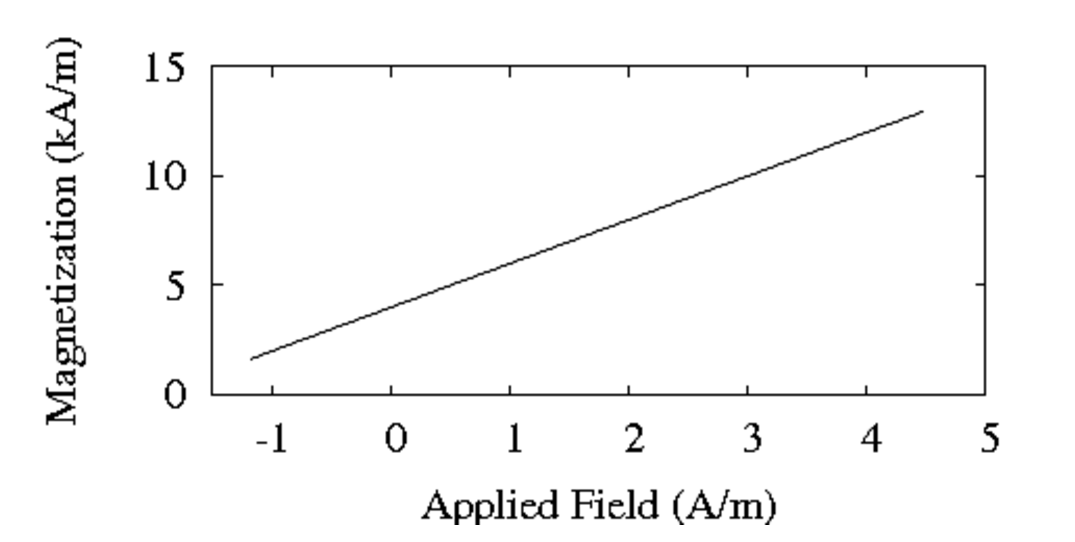
\includegraphics[width=70mm]{Fig1-Times-Roman.eps}
%\includegraphics[width=70mm]{Fig1-TimesNewRomanPSMT.eps}
%\fbox{ \rule[-17mm]{0pt}{30mm} FIGURE }
\end{center}
\caption{Magnetization as a function of applied field.}
\vspace*{-3pt}
{\hfill\footnotesize Note how the caption is centered in the column.\hfill}
\end{figure}

Figure axis labels are often a source of confusion. Use words rather
than symbols.  For example, write ``Magnetization,'' or
``Magnetization (M)'' not just ``M.''  Put units in parentheses.  Do
not label axes only with units.  In the example, write ``Magnetization
(A/m)'' or ``Magnetization (A $\cdot$ m$^{-1}$).''  Do not label axes
with a ratio of quantities and units.  For example, write
``Temperature (K),'' not ``Temperature/K.''

Multipliers can be especially confusing.  Write ``Magnetization
(kA/m)'' or ``Magnetization ($10^3$ A/m).''  Figure labels should be
legible, about 10-point type.

\subsection{References}
Number citations consecutively in square brackets [1].  Punctuation
follows the bracket [2]. Refer simply to the reference number, as in
[3]. Use ``Ref. [3]'' or ``Reference [3]'' at the beginning of a
sentence: ``Reference [3] was the first ...''


Gather the full set of references together in the section of
references.  Place the section of references before any appendices,
unless they contain references.  Arrange the references in
alphabetical order or in order of appearance in the paper.

Give all authors' names; use ``et al.''  if there are six authors or
more.  Papers that have not been published, even if they have been
submitted for publication, should be cited as ``unpublished'' [4].
Papers that have been accepted for publication should be cited as ``in
press'' [5].  In a paper title, capitalize the first word and all
other words except for conjunctions, prepositions less than seven
letters, and prepositional phrases.

For papers published in translated journals, first give the English
citation, then the original foreign-language citation [6].

\subsection{Appendices}
Although conference papers do not normally have an appendix,
appendices, if any, directly follow the text and the references, (but
see IV.B).  Letter them in sequence and provide an informative title:
{\bf Appendix A Title of Appendix}.

\subsection{Footnote}
Number footnotes separately in superscripts like this\footnote{This is
  how a footnote should appear.}.  Place the actual footnote at the
bottom of the column in which it was cited.  Footnotes should be
separated from the text by a line\footnote{Note the line separating
  the footnotes from the text.}.  Do not put footnotes in the
reference list.  Use letters for table footnotes (see Table I).


\subsection{Abbreviations and Acronyms}

Define abbreviations and acronyms the first time they are used in the
text, even if they have been defined in the abstract.  Abbreviations
such as APSIPA, SI, MKS, CGS, ac, dc, and rms do not have to be defined.
Do not use abbreviations in the title unless they are unavoidable.

\subsection{Equations}

Number equations consecutively with equation numbers in parentheses
flush with the right margin, as in (1).  To make your equations more
compact, you may use the solidus ( / ), the exp function, or
appropriate exponents.  Italicize Roman symbols for quantities and
variables, but not Greek symbols.  Use an en dash ( $-$ ) rather than
a hyphen for a minus sign.  Use parentheses to avoid ambiguities in
denominators.  Punctuate equations with commas or periods when they
are part of a sentence, as in

\begin{equation}
 a + b = c.
\end{equation}

Symbols in your equation should be defined before the equation appears
or immediately following.  Use ``(1),'' not ``Eq. (1)'' or ``equation
(1),'' except at the beginning of a sentence: ``Equation (1) is ...''

\subsection{Other Recommendations}

The Roman numerals used to number the section headings are optional.
If you do use them, do not number {\scshape{Acknowledgment}} and
{\scshape{References}}, and begin Subheadings with letters.

Use two spaces after periods (full stops).  Hyphenate complex
modifiers: ``zero-field-cooled magnetization.''  Avoid dangling
participles, such as, ``Using (1), the potential was calculated.''
Write instead, ``The potential was calculated using (1),'' or ``Using
(1), we calculated the potential.''


\renewcommand{\textheight}{98mm}


Use a zero before decimal points: ``0.25,'' not ``.25.''  Use
``cm$^3$,'' not ``cc.''  Do not mix complete spellings and
abbreviations of units: ``Wb/m$^2$'' or ``webers per square meter,''
not ``webers/m$^2$.''  Spell units when they appear in text: ``...a
few henries,'' not ``...a few H.''  If your native language is not
English, try to get a native English-speaking colleague to proofread
your paper.  Do not add page numbers.

%\newpage
\section{Units}

Use either SI (MKS) or CGS as primary units. (SI units are
encouraged.) English units may be used as secondary units (in
parentheses). An exception would be the use of English units as
identifiers in trade, such as ``3.5-inch disk drive.''

Avoid combining SI and CGS units, such as current in amperes and
magnetic field in oersteds. This often leads to confusion because
equations do not balance dimensionally. If you must use mixed units,
clearly state the units for each quantity that you use in an equation.

\section{Some Common Mistakes}

The word ``data'' is plural, not singular.  The subscript for the
permeability of vacuum$_0$ is zero, not a lowercase letter ``o.''  In
American English, periods and commas are within quotation marks,
``like this period.''  A parenthetical statement at the end of a
sentence is punctuated outside of the closing parenthesis (like this).
(A parenthetical \emph{sentence} is punctuated within the
parentheses.)  A graph within a graph is an ``inset,'' not an
``insert.''  The word alternatively is preferred to the word
``alternately'' (unless you mean something that alternates).  Do not
use the word ``essentially'' to mean ``approximately'' or
``effectively.''  Be aware of the different meanings of the homophones
``affect'' and ``effect,'' ``complement'' and ``compliment,''
``discreet'' and ``discrete,'' ``principal'' and ``principle.''  Do
not confuse ``imply'' and ``infer.''  The prefix ``non'' is not a
word; it should be joined to the word it modifies, usually without a
hyphen.  There is no period after the ``et'' in the Latin abbreviation
``et al.''  The abbreviation ``i.e.''  means ``that is,'' and the
abbreviation ``e.g.''  means ``for example.''  An excellent style
manual for science writers is [7].


\section{Conclusions}
The conclusion goes here.

\section*{Acknowledgment}

The preferred spelling of the word ``acknowledgment'' in America is
without an ``e'' after the ``g.''  Try to avoid the stilted
expression, ``One of us (R. B. G.) thanks ...'' Instead, try
``R.B.G. thanks ...''  Put sponsor acknowledgments in the unnumbered
footnote on the first page.

\begin{thebibliography}{1}

\bibitem{1}
G.~Eason, B.~Noble, and I.~N.~Sneddon, ``On certain integrals of
Lipschitz-Hankel type involving products of Bessel functions,''
\emph{Phil. Trans. Roy. Soc. London,} vol. A247, pp. 529-551, April
1955.

\bibitem{2}
J.~Clerk~Maxwell, \emph{A Treatise on Electricity and Magnetism,}
3$^{\rm rd}$ ed., vol. 2. Oxford: Clarendon, 1892, pp.68-73.

\bibitem{3}
I.~S.~Jacobs and C.~P.~Bean, ``Fine particles, thin films and exchange
anisotropy,'' in \emph{Magnetism,} vol. III, G.T. Rado and H. Suhl,
Eds. New York: Academic, 1963, pp. 271-350.

\bibitem{4}
K.~Elissa, ``Title of paper if known,'' unpublished.

\bibitem{5}
R.~Nicole, ``Title of paper with only first word capitalized,''
\emph{J. Name Stand. Abbrev.,} in press.

\bibitem{6}
Y.~Yorozu, M.~Hirano, K.~Oka, and Y.~Tagawa, ``Electron spectroscopy
studies on magneto-optical media and plastic substrate interface,''
\emph{APSIPA Transl. J. Magn. Japan,} vol. 2, pp. 740-741, August 1987
[\emph{Digests 9$^{\rm th}$ Annual Conf. Magnetics Japan,} p. 301,
1982].

\bibitem{7}
M.~Young, \emph{The Technical Writer's Handbook.} Mill Valley, CA:
University Science, 1989.

\end{thebibliography}
\end{document}
